% =============================================================================
%  MINIREVIEW: LLM Applications in Bioinformatics
%  MU Bioinformática · Universidad Nebrija · Iniciación en la Investigación
%  Compilación:  pdflatex → bibtex → pdflatex → pdflatex  (4 pasos)
%  En Overleaf:  seleccionar pdfLaTeX como compilador (menú → Settings).
% =============================================================================

\documentclass[12pt,a4paper]{article}

% --- Codificación y tipografía -----------------------------------------------
\usepackage[utf8]{inputenc}
\usepackage[T1]{fontenc}
\usepackage{lmodern}
\usepackage{microtype}
% \usepackage[spanish]{babel} % Opcional: activar si el idioma esta instalado en TinyTeX.

% --- Página ------------------------------------------------------------------
\usepackage{geometry}
\geometry{left=25mm, right=25mm, top=30mm, bottom=30mm}
\usepackage{setspace}\onehalfspacing
% \usepackage[left]{lineno}\linenumbers   % Descomentar para revisión (doble numeración)

% --- Matemáticas -------------------------------------------------------------
\usepackage{amsmath,amssymb}
\usepackage{siunitx}
\sisetup{group-separator={,}}

% --- Figuras y subfiguras ----------------------------------------------------
\usepackage{graphicx}\graphicspath{{../figures/}}
\usepackage[font=small,labelfont=bf,labelsep=period]{caption}
\usepackage{subcaption}

% --- Tablas ------------------------------------------------------------------
\usepackage{booktabs,array,multirow,longtable}
\usepackage{tabularx}
\newcolumntype{Y}{>{\centering\arraybackslash}X}

% --- Listas ------------------------------------------------------------------
\usepackage{enumitem}\setlist{nosep}

% --- Código fuente -----------------------------------------------------------
\usepackage{listings}
\lstset{
  basicstyle       = \small\ttfamily,
  keywordstyle     = \bfseries\color{blue!70!black},
  commentstyle     = \itshape\color{gray},
  stringstyle      = \color{red!60!black},
  numberstyle      = \tiny\color{gray},
  numbers          = left,
  numbersep        = 6pt,
  frame            = single,
  framerule        = 0.4pt,
  rulecolor        = \color{black!30},
  backgroundcolor  = \color{black!3},
  breaklines       = true,
  showstringspaces = false,
  tabsize          = 4,
  captionpos       = b,
  aboveskip        = 10pt,
  belowskip        = 6pt,
}
\lstdefinestyle{python}{language=Python,
  morekeywords={as,with,True,False,None}}
\lstdefinestyle{R}{language=R,
  morekeywords={library,function,if,else,for,in,TRUE,FALSE,NULL}}
\lstdefinestyle{bash}{language=bash,
  morekeywords={snakemake,conda,pip}}

% --- Cajas destacadas (tipo Box de Nature Reviews) ---------------------------
\usepackage{tcolorbox}
\newtcolorbox{infobox}[1][]{
  colback=blue!3, colframe=blue!40!black,
  fonttitle=\bfseries, coltitle=white, colbacktitle=blue!40!black,
  boxrule=0.5pt, arc=2pt, left=6pt, right=6pt, title={#1}}
\newtcolorbox{keypoint}[1][]{
  colback=yellow!5, colframe=orange!60!black,
  fonttitle=\bfseries,
  boxrule=0.4pt, arc=2pt, left=6pt, right=6pt, title={#1}}

% --- TikZ (diagramas) -------------------------------------------------------
\usepackage{tikz}
\usetikzlibrary{shapes.geometric,arrows.meta,positioning,calc}

% --- Hipervínculos -----------------------------------------------------------
\usepackage[colorlinks,
            linkcolor=black,
            citecolor=blue!60!black,
            urlcolor=blue!60!black]{hyperref}
\usepackage[capitalise,noabbrev]{cleveref}

% --- Bibliografía: BibTeX clásico con natbib ---------------------------------
\usepackage[numbers,sort&compress]{natbib}
\bibliographystyle{unsrtnat}

% --- Comandos personalizados -------------------------------------------------
\newcommand{\gene}[1]{\textit{#1}}
\newcommand{\tool}[1]{\textsc{\lowercase{#1}}}
\newcommand{\pvalue}{\ensuremath{p}}
\newcommand{\padj}{\ensuremath{p_{\text{adj}}}}
\newcommand{\foldchange}{\ensuremath{\log_2\text{FC}}}

% --- Metadatos ---------------------------------------------------------------
\title{Sistemas basados en agentes y modelos de lenguaje (LLMs) para la
automatización de workflows en bioinformática: arquitecturas, aplicaciones y
desafíos}
\author{Jose Camacho%
  \thanks{Máster en Bioinformática, Universidad Nebrija.}}
\date{06 Mayo 2026}

% =============================================================================
\begin{document}
\maketitle

% --- Resumen -----------------------------------------------------------------
\begin{abstract}\noindent
Los modelos de lenguaje de gran escala (LLMs) han abierto nuevas posibilidades
para automatizar tareas complejas en bioinformática, pero su naturaleza
probabilística limita su uso directo en workflows científicos que requieren
trazabilidad, precisión y reproducibilidad. Esta mini-review analiza 15 estudios
recientes sobre sistemas basados en agentes aplicados a transcriptómica,
\textit{single-cell omics}, modelado farmacocinético, descubrimiento terapéutico,
visualización científica y generación automatizada de protocolos. La evidencia
revisada muestra una transición desde enfoques basados únicamente en
\textit{prompting} hacia arquitecturas agénticas capaces de planificar tareas,
invocar herramientas externas, ejecutar código, autocorregirse y coordinar
múltiples agentes especializados. Los principales hallazgos señalan que la
orquestación jerárquica, el \textit{grounding}, la observabilidad y los
protocolos de interoperabilidad como el Model Context Protocol (MCP) son
elementos centrales para escalar estos sistemas de forma robusta. No obstante,
persisten desafíos importantes relacionados con alucinaciones, coste
computacional, propagación de errores, ausencia de benchmarks estandarizados y
gobernanza científica. En conjunto, los sistemas agénticos representan un cambio
de paradigma: no solo automatizan tareas repetitivas, sino que pueden actuar
como copilotos científicos capaces de ampliar el acceso a workflows
bioinformáticos complejos bajo supervisión humana.
\medskip\noindent
\textbf{Palabras clave:} modelos de lenguaje de gran escala, sistemas
agénticos, bioinformática, automatización, workflows, reproducibilidad,
gobernanza
\end{abstract}

\newpage\tableofcontents\newpage

% --- Secciones principales ---------------------------------------------------
% ==============================================================================
% SECTION 1: INTRODUCTION
% ==============================================================================
% Extensión: 400–600 palabras
% Estructura embudo: contexto general → estado del arte → brecha de conocimiento → objetivo
% Tiempo: presente para hechos generales, pasado para estudios previos
% Incluye: citas con natbib, ecuaciones inline, números formateados (\num{}),
% párrafo guía con referencias cruzadas (\Cref)

\section{Introducción}\label{sec:intro}

La bioinformática contemporánea depende de workflows compuestos por múltiples
herramientas, formatos de archivo y decisiones analíticas que rara vez siguen
una trayectoria completamente lineal. Aunque los pipelines tradicionales han
permitido estandarizar tareas como alineamiento, cuantificación, anotación o
modelado, su ejecución sigue exigiendo intervención humana para adaptar
parámetros, resolver errores, encadenar software heterogéneo y reinterpretar
resultados intermedios. Esta fricción se vuelve más evidente en contextos como
la transcriptómica, las ómicas de célula única o la farmacometría, donde la
complejidad técnica crece al mismo ritmo que el volumen de datos.

En ese escenario, los modelos de lenguaje de gran escala (LLMs) han comenzado a
desempeñar un papel distinto al de asistentes conversacionales genéricos.
Cuando se integran en sistemas capaces de planificar, invocar herramientas,
ejecutar código y corregir errores a partir de la retroalimentación del
entorno, los LLMs pasan de ser interfaces de \textit{prompting} a componentes
de arquitecturas agénticas orientadas a la automatización
científica~\citep{42042548,41912700}. Esta evolución ha favorecido agentes que
operan sobre notebooks, APIs, bases de datos, software bioinformático y
servicios web.

Sin embargo, el interés creciente por estos sistemas no ha venido acompañado de
un marco sintético claro para describir cómo están siendo diseñados, evaluados
y limitados dentro del dominio bioinformático. La literatura reciente incluye
agentes recursivos, sistemas multi-agente, asistentes con \textit{grounding} y
plataformas con observabilidad, pero persisten preguntas sobre
reproducibilidad, coste computacional, trazabilidad, control humano e
interoperabilidad. El campo avanza rápido en prototipos y demostraciones, pero
todavía carece de una visión ordenada de sus arquitecturas dominantes y de sus
condiciones de validez científica.

Esta mini-review examina 15 estudios publicados en 2025 y 2026 sobre el uso de
LLMs y sistemas basados en agentes para la automatización de workflows en
bioinformática. La Sección~\ref{sec:methods} describe la estrategia de búsqueda
y los criterios de selección; la Sección~\ref{sec:synthesis} organiza la
evidencia en cuatro ejes temáticos; la Sección~\ref{sec:discussion} discute los
hallazgos, limitaciones y vacíos de la literatura; y la
Sección~\ref{sec:conclusions} presenta las conclusiones y perspectivas futuras
del área.

% ==============================================================================
% SECTION 2: SEARCH METHODOLOGY
% ==============================================================================
% Extensión: 300–500 palabras
% Estructura: pregunta PICO, bases de datos, ecuación de búsqueda,
% criterios de inclusión/exclusión, diagrama PRISMA (TikZ)

\section{Metodología de búsqueda}\label{sec:methods}

\subsection{Pregunta de investigación}

Se formuló una pregunta de investigación basada en el marco PICO:

¿Qué tan efectivos son los sistemas basados en Large Language Models (LLMs) y 
agentes en comparación con workflows tradicionales para la automatización de 
pipelines bioinformáticos?

\begin{table}[htbp]
  \centering
  \caption{Marco PICO de la pregunta de investigación.}\label{tab:pico}
  \begin{tabular}{@{}p{3.2cm} p{9.2cm}@{}}
    \toprule
    \textbf{Componente} & \textbf{Descripción} \\
    \midrule
    \textbf{P: Población}    & Pipelines bioinformáticos, incluyendo análisis de RNA-seq, genómica y transcriptómica. \\
    \textbf{I: Intervención} & Sistemas basados en Large Language Models (LLMs) y agentes. \\
    \textbf{C: Comparación}   & Workflows tradicionales, tales como scripts manuales y pipelines estáticos. \\
    \textbf{O: Resultado}      & Nivel de automatización, eficiencia, reproducibilidad y control del flujo de trabajo. \\
    \bottomrule
  \end{tabular}
\end{table}

\subsection{Bases de datos y estrategia de búsqueda}

La búsqueda se realizó en PubMed, complementada con repositorios académicos 
y plataformas de preprints, abarcando publicaciones entre 2020 y 2026. La 
estrategia se ejecutó el 5 de mayo de 2026 mediante la siguiente ecuación:

\begin{quote}\footnotesize\ttfamily\raggedright
("large language models"[TIAB] OR LLM OR "AI agents") \\
\hspace*{1em}AND ("bioinformatics" OR "RNA-seq" OR "genomics") \\
\hspace*{1em}AND ("workflow" OR "pipeline" OR "automation" OR "agent" OR "orchestration")
\end{quote}

Se seleccionaron estudios enfocados en la orquestación de flujos de trabajo y 
sistemas agénticos, integrando adicionalmente documentación técnica sobre 
marcos de trabajo como LangChain y fundamentos de agentes para sustentar el 
análisis arquitectónico.

\subsection{Criterios de inclusión y exclusión}

\paragraph{Criterios de inclusión}

\begin{itemize}
  \item Estudios que describieran arquitecturas explícitas basadas en agentes, incluyendo planificación, uso de herramientas externas o sistemas multi-agente.
  \item Aplicaciones directas en bioinformática, tales como genómica, transcriptómica, proteómica o diseño automatizado de protocolos.
  \item Artículos que analizaran desafíos técnicos asociados al uso de LLMs y agentes, incluyendo alucinaciones, reproducibilidad, coste computacional o control de ejecución.
  \item Publicaciones que propusieran benchmarks, métricas o estrategias de evaluación para sistemas basados en agentes.
\end{itemize}

\paragraph{Criterios de exclusión}

\begin{itemize}
  \item Estudios enfocados exclusivamente en aplicaciones clínicas o diagnóstico por imagen sin relación con workflows bioinformáticos.
  \item Trabajos que utilizaran LLMs únicamente mediante prompting simple, sin capacidades de planificación, uso de herramientas o ejecución autónoma.
  \item Artículos centrados en aplicaciones médicas no relacionadas con bioinformática computacional, incluyendo encuestas de satisfacción de pacientes, medicina tradicional china o estudios clínicos sin componente de automatización de workflows.
  \item Publicaciones sin descripción metodológica clara o sin relación directa con infraestructura computacional basada en agentes.
\end{itemize}

\subsection{Selección de estudios}

La búsqueda inicial recuperó 40 artículos de PubMed. El cribado de títulos,
resúmenes y conclusiones excluyó estudios sobre aplicaciones clínicas,
\textit{prompting} simple o medicina no computacional. Tras aplicar los
criterios de inclusión, se seleccionaron 15 artículos para la síntesis
cualitativa (\cref{fig:prisma}).

Para complementar el análisis de las arquitecturas implementadas en dichos
artículos, se integró de forma dirigida la documentación técnica de LangChain,
la cual sirvió como marco de referencia para fundamentar los componentes de
diseño de agentes, memoria y uso de herramientas discutidos en esta
revisión~\citep{LangChainAgents2026,LangChainMemory2026,LangChainTools2026}.

\begin{figure}[htbp]
  \centering
  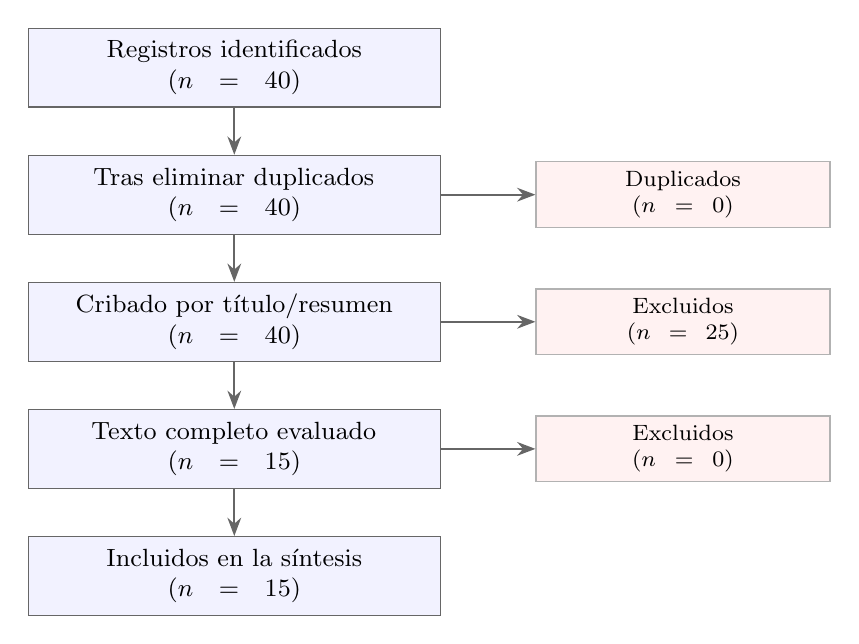
\begin{tikzpicture}[
      box/.style  = {rectangle, draw=black!60, fill=blue!5,
                     text width=5cm, minimum height=1cm,
                     align=center, font=\small},
      arrow/.style = {-Stealth, thick, black!60},
      excl/.style  = {rectangle, draw=black!30, fill=red!5,
                      text width=3.5cm, minimum height=0.8cm,
                      align=center, font=\footnotesize}
    ]
    \node[box] (id)     {Registros identificados\\($n = 40$) };
    \node[box, below=0.6cm of id]  (dedup)  {Tras eliminar duplicados\\($n = 40$) };
    \node[box, below=0.6cm of dedup](screen) {Cribado por título/resumen\\($n = 40$) };
    \node[box, below=0.6cm of screen](full)  {Texto completo evaluado\\($n = 15$) };
    \node[box, below=0.6cm of full] (incl)   {Incluidos en la síntesis\\($n = 15$) };

    \node[excl, right=1.2cm of dedup]  (e1) {Duplicados\\($n = 0$) };
    \node[excl, right=1.2cm of screen] (e2) {Excluidos\\($n = 25$) };
    \node[excl, right=1.2cm of full]   (e3) {Excluidos\\($n = 0$) };

    \draw[arrow] (id)     -- (dedup);
    \draw[arrow] (dedup)  -- (screen);
    \draw[arrow] (screen) -- (full);
    \draw[arrow] (full)   -- (incl);
    \draw[arrow] (dedup.east)  -- (e1.west);
    \draw[arrow] (screen.east) -- (e2.west);
    \draw[arrow] (full.east)   -- (e3.west);
  \end{tikzpicture}
  \caption{Diagrama de flujo PRISMA del proceso de selección de estudios.}
  \label{fig:prisma}
\end{figure}

% ==============================================================================
% SECTION 3: THEMATIC SYNTHESIS
% ==============================================================================
% Extensión: 2000–3000 palabras
% Estructura: tabla de extracción (longtable), subsecciones por tema,
% ecuaciones display (equation, align, cases), cajas destacadas (infobox, keypoint),
% listings de código (Python, R, bash), tablas comparativas (tabularx)

\section{Síntesis temática}\label{sec:synthesis}

% --- RESUMEN GENERAL ---
Los 15 estudios seleccionados fueron analizados y categorizados en cuatro ejes
temáticos que abordan desde el diseño estructural hasta la validación científica
de los sistemas. La \cref{subsec:architectures} examina las arquitecturas
agénticas; la \cref{subsec:pipeline-automation} analiza la automatización de
pipelines específicos, incluyendo genómica, scRNA-seq y farmacometría; la
\cref{subsec:reproducibility} evalúa las estrategias de reproducibilidad y
benchmarking; y finalmente, la \cref{subsec:governance} discute las limitaciones
técnicas y los marcos de gobernanza.

La \cref{tab:extraction} sintetiza las características operativas, aplicaciones
clave y hallazgos principales de la evidencia analizada, sirviendo como base
para la discusión técnica subsiguiente.

\begin{enumerate}
  \item Arquitecturas agénticas y patrones de orquestación.
  \item Automatización de pipelines bioinformáticos específicos.
  \item Reproducibilidad, benchmarking y evaluación comparativa.
  \item Limitaciones técnicas, supervisión humana y gobernanza.
\end{enumerate}


% --- TABLA DE EXTRACCIÓN (OBLIGATORIA) ---
% Longtable permite que la tabla continúe en varias páginas
\begin{longtable}{p{3.0cm} p{2.8cm} p{2.7cm} p{3.5cm} p{2.6cm}}
\caption{Tabla de extracción de datos de los estudios incluidos.}
\label{tab:extraction}\\
\toprule
\textbf{Autor, año} & \textbf{Enfoque} & \textbf{Aplicación} &
\textbf{Hallazgo clave} & \textbf{Limitación} \\
\midrule\endfirsthead
\multicolumn{5}{l}{\small\itshape Continuación de la página anterior}\\
\toprule
\textbf{Autor, año} & \textbf{Enfoque} & \textbf{Aplicación} &
\textbf{Hallazgo clave} & \textbf{Limitación} \\
\midrule\endhead
\midrule\multicolumn{5}{r}{\small\itshape Continúa en la página siguiente}\\\endfoot
\bottomrule\endlastfoot

\textit{Artificial Intelligence in Transcriptomics}, 2026 &
Modelo IURA &
Transcriptómica &
Transición hacia sistemas autónomos &
Marco emergente \\
\addlinespace
\textit{BioMedAgent}, 2026 &
Framework multi-agente &
Workflows bioinformáticos &
Selección autónoma y encadenamiento de tareas &
Alto coste computacional \\
\addlinespace
\textit{PKGPT}, 2026 &
Agente recursivo basado en LLMs &
Modelado farmacocinético &
Refinamiento iterativo mediante software externo &
Requiere supervisión experta para plausibilidad e interpretabilidad \\
\addlinespace
\textit{ChatSpatial}, 2026 &
Orquestación basada en esquemas &
Transcriptómica espacial &
Reproducibilidad entre workflows R/Python &
Preprint; validación todavía emergente \\
\addlinespace
\textit{CellVoyager}, 2026 &
Agente autónomo &
Análisis de datos biológicos &
Ejecución autónoma de análisis y hallazgos en notebooks &
La interpretación final sigue requiriendo revisión experta \\
\addlinespace
\textit{Virtual Biotech}, 2026 &
Sistema jerárquico multi-agente &
Descubrimiento terapéutico &
Orquestación científica de punta a punta &
Preprint; evidencia aún preliminar \\
\addlinespace
\textit{Benchmarking LLM-based Agents}, 2026 &
Framework de benchmarking &
Ómicas de célula única &
Evaluación de capacidades agénticas en análisis ómicos &
Benchmarks limitados \\
\addlinespace
\textit{MCPmed}, 2026 &
Arquitectura basada en MCP &
Servicios web bioinformáticos &
Interoperabilidad entre agentes y servicios web bioinformáticos &
Propuesta temprana \\
\addlinespace
\textit{Reliable Data Science Copilots}, 2026 &
Refinamiento iterativo &
Programación científica &
Necesidad de validación iterativa &
Baja precisión inicial sin refinamiento \\
\addlinespace
\textit{Metaviral Workflow Generation}, 2026 &
Generación automática de pipelines &
Virología computacional &
Automatización de workflows multi-step &
Riesgo de alucinaciones \\
\addlinespace
\textit{ggplotAgent}, 2026 &
Agente auto-correctivo &
Visualización científica &
Corrección autónoma de errores &
Alcance limitado \\
\addlinespace
\textit{Functional Genomics Assistant}, 2025 &
Asistente basado en evidencia &
Genómica funcional &
Mejora trazabilidad y procedencia &
Requiere fuentes curadas \\
\addlinespace
\textit{Multi-Agent AI Systems Review}, 2026 &
Survey / taxonomía &
Datos biológicos y clínicos &
Tendencias en arquitecturas multi-agente &
Evidencia mayormente teórica \\
\addlinespace
\textit{AI Agents for Biological Research}, 2026 &
Framework taxonómico 5D &
Automatización científica &
Clasificación estructurada de sistemas agénticos &
Validación experimental limitada \\
\addlinespace
\textit{Automated Protein Protocol Optimization}, 2026 &
Automatización basada en LLMs &
Protocolos de proteínas &
Traducción de literatura a protocolos ejecutables &
Desafíos de integración wet-lab \\
\end{longtable}


% --- SUBSECCIÓN 1 ---
\subsection{Arquitecturas agénticas y patrones de orquestación}\label{subsec:architectures}

Trabajos como \textit{BioMedAgent}~\citep{41912700} y
\textit{PKGPT}~\citep{42076151} mostraron que es posible
integrar herramientas bioinformáticas externas dentro de arquitecturas capaces
de ejecutar workflows complejos y refinar sus resultados de manera iterativa,
aunque todavía bajo supervisión humana en tareas de alta exigencia técnica. De
forma similar, \textit{MCPmed}~\citep{41729821} propuso mecanismos de
interoperabilidad entre agentes y servicios web bioinformáticos mediante
protocolos estructurados, destacando la necesidad de infraestructuras
estandarizadas para sistemas científicos autónomos.

Asimismo, varios estudios identificaron patrones arquitectónicos comunes,
incluyendo sistemas jerárquicos multi-agente, agentes recursivos de refinamiento
y modelos orientados a la orquestación de tareas científicas complejas.

Es importante precisar que esta caracterización arquitectónica no se basa
únicamente en los artículos empíricos incluidos, sino también en una capa
teórica de apoyo sobre diseño de agentes, memoria y uso de herramientas. Por
ello, aunque los trabajos centrados exclusivamente en \textit{prompting} simple
fueron excluidos del corpus principal, el nivel de LLM base se conserva aquí
como referencia conceptual para mostrar el salto estructural hacia sistemas con
planificación, estado y ejecución externa. En ese puente conceptual, la
documentación oficial de LangChain resulta útil para describir de manera
estandarizada cómo se articulan los componentes mínimos de un agente moderno,
incluyendo el ciclo modelo-herramientas, la memoria operativa y la interacción
con funciones externas~\citep{LangChainAgents2026,LangChainMemory2026,LangChainTools2026}.

Esta evolución arquitectónica se puede categorizar en tres estadios
(\cref{fig:agentic-levels}). Inicialmente, los sistemas operaban mediante
\textit{prompting} directo (Nivel 1). La introducción de frameworks como
LangChain permitió el desarrollo de agentes con capacidad de razonamiento y uso
de herramientas (Nivel 2), donde el LLM actúa como un motor de decisiones para
ejecutar software bioinformático. Finalmente, la frontera actual se desplaza
hacia sistemas multi-agente jerárquicos (Nivel 3), donde un supervisor
coordina agentes especializados y distribuye subtareas científicas complejas,
como se observa en propuestas recientes como \textit{Virtual
Biotech}~\citep{41808990} \textit{(preprint)} y en marcos de interoperabilidad
como \textit{MCPmed}~\citep{41729821}.

\begin{figure}[htbp]
  \centering
  \begin{subfigure}[t]{0.47\textwidth}
    \centering
    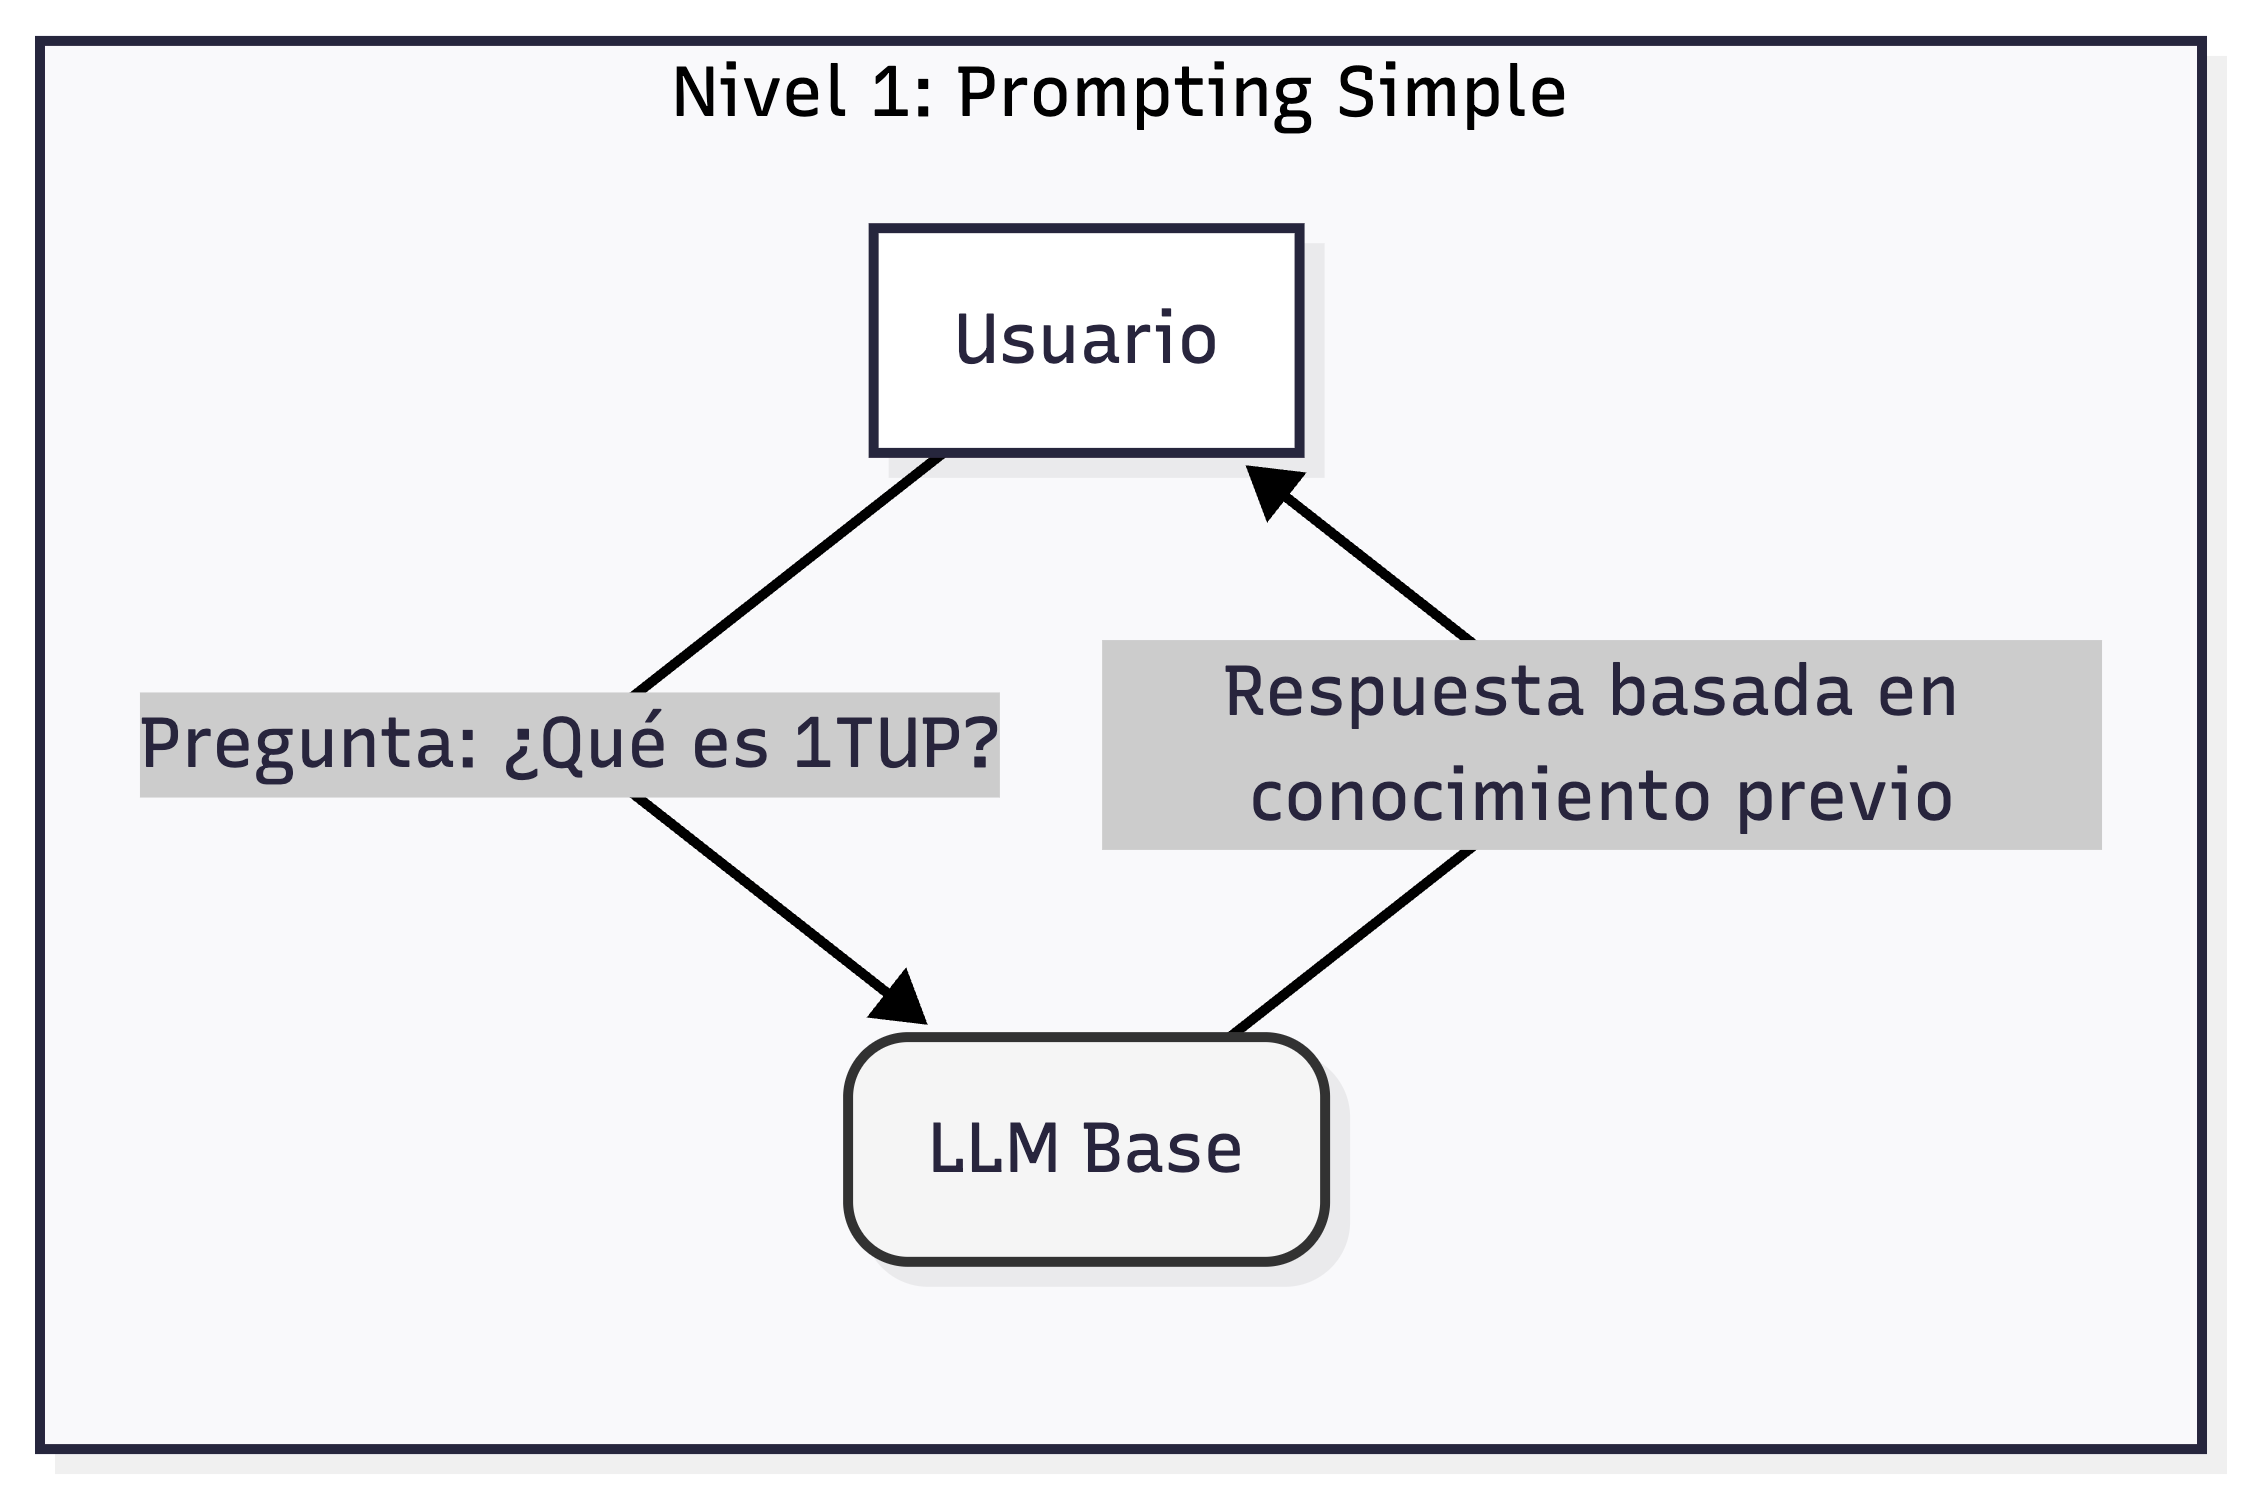
\includegraphics[width=\linewidth]{llm_base.png}
    \caption{LLM base}
    \label{fig:llm-base}
  \end{subfigure}\hfill
  \begin{subfigure}[t]{0.47\textwidth}
    \centering
    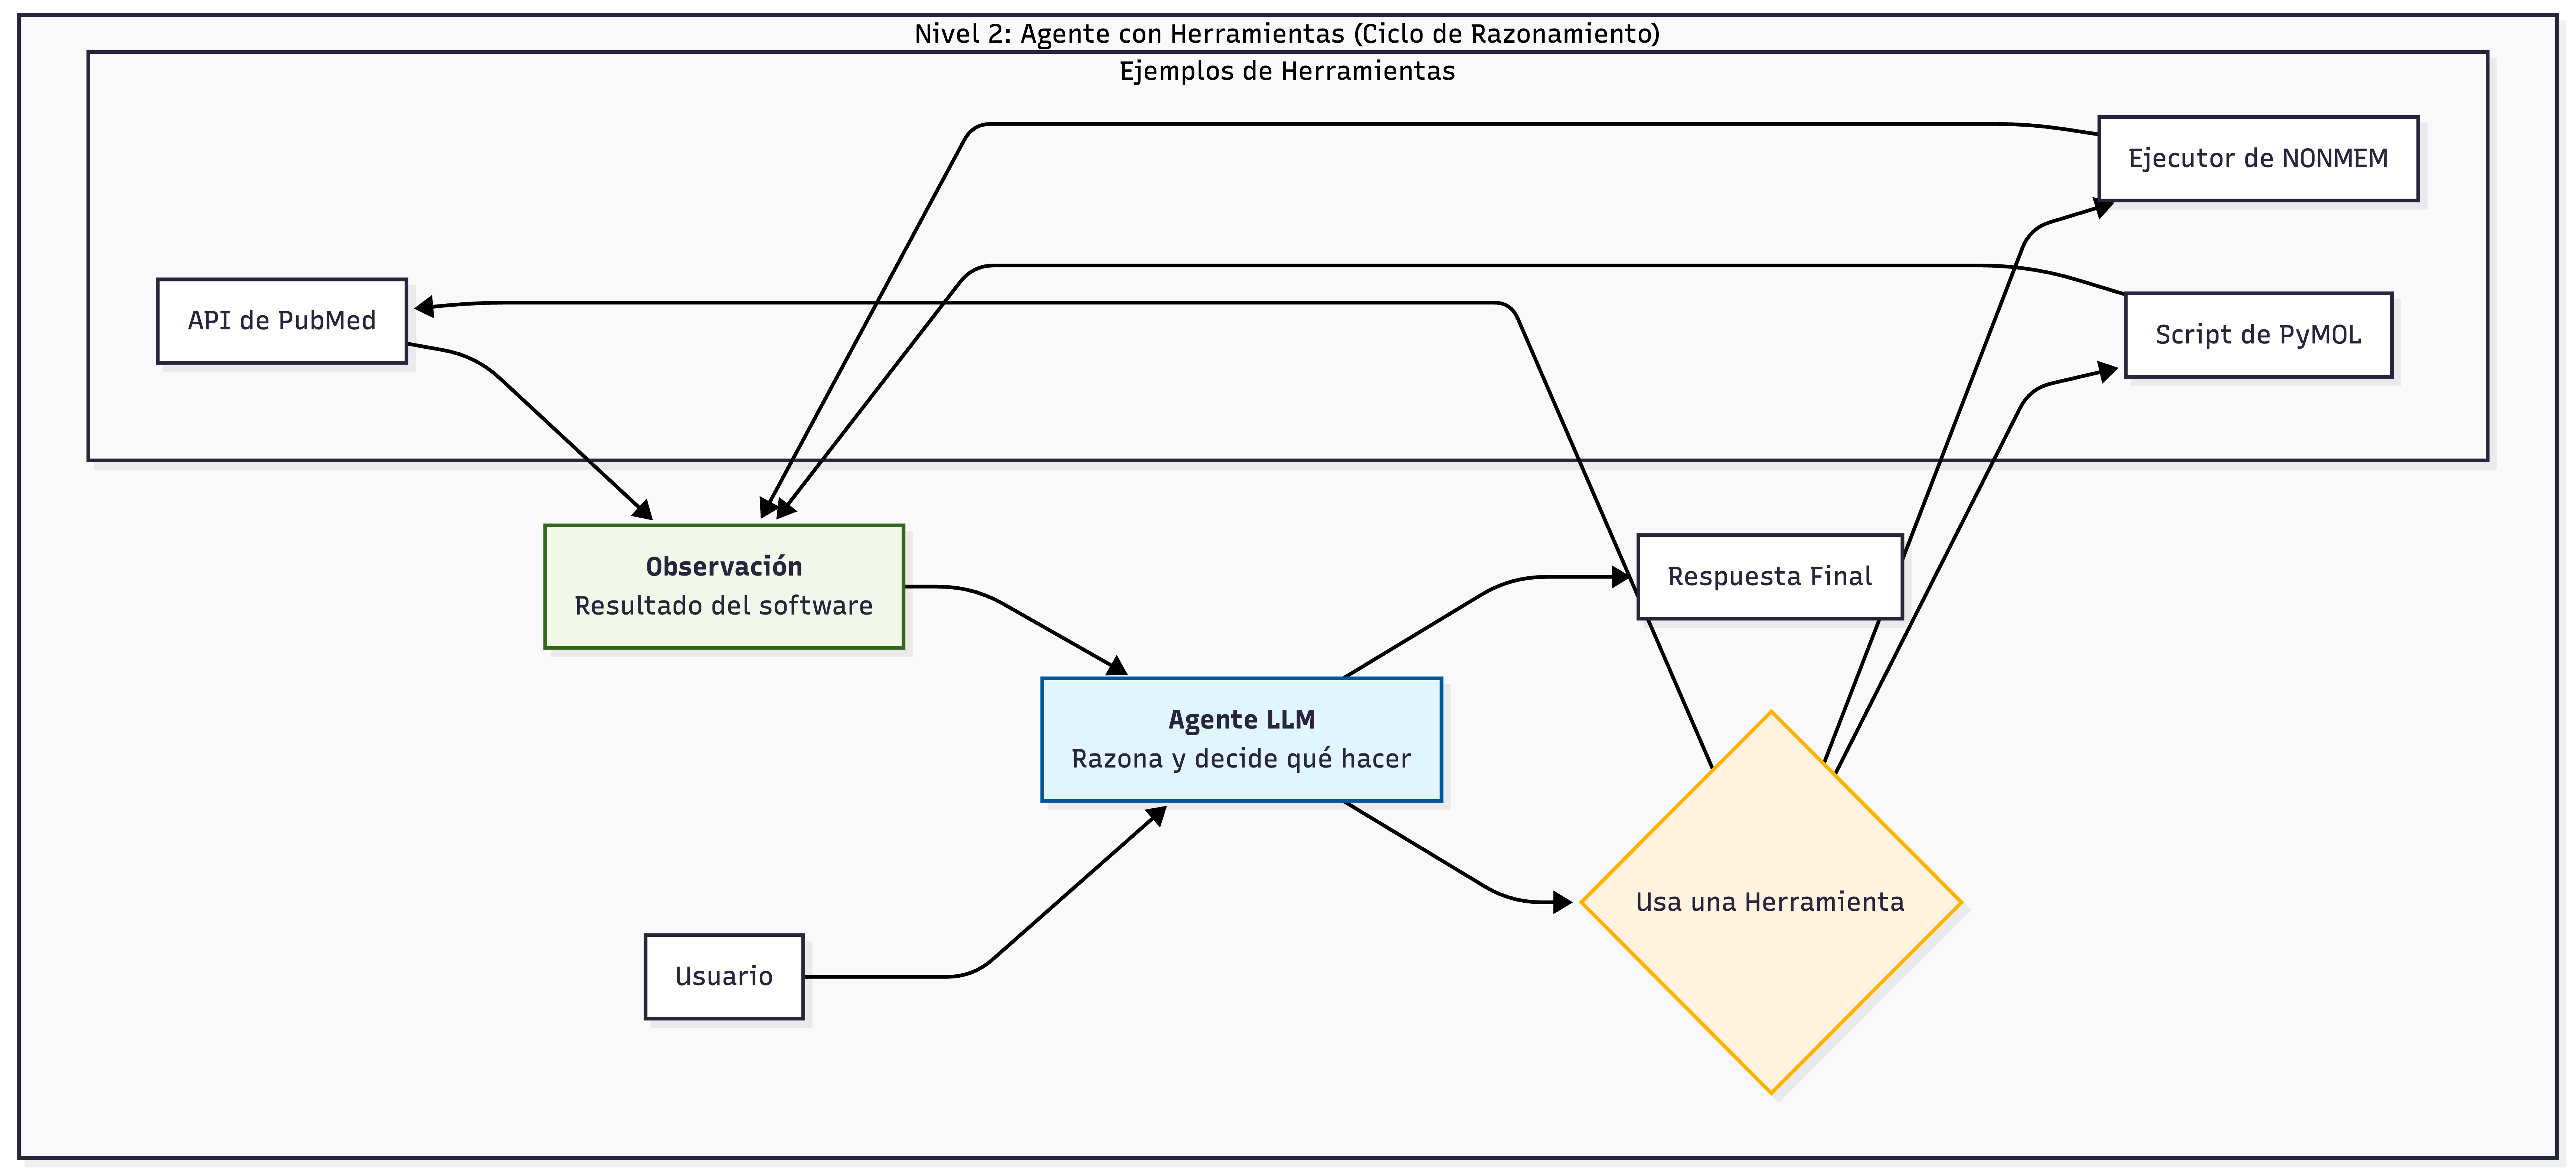
\includegraphics[width=\linewidth]{agente.png}
    \caption{Agente con herramientas}
    \label{fig:agent-tool-use}
  \end{subfigure}

  \vspace{0.8em}

  \begin{subfigure}[t]{0.72\textwidth}
    \centering
    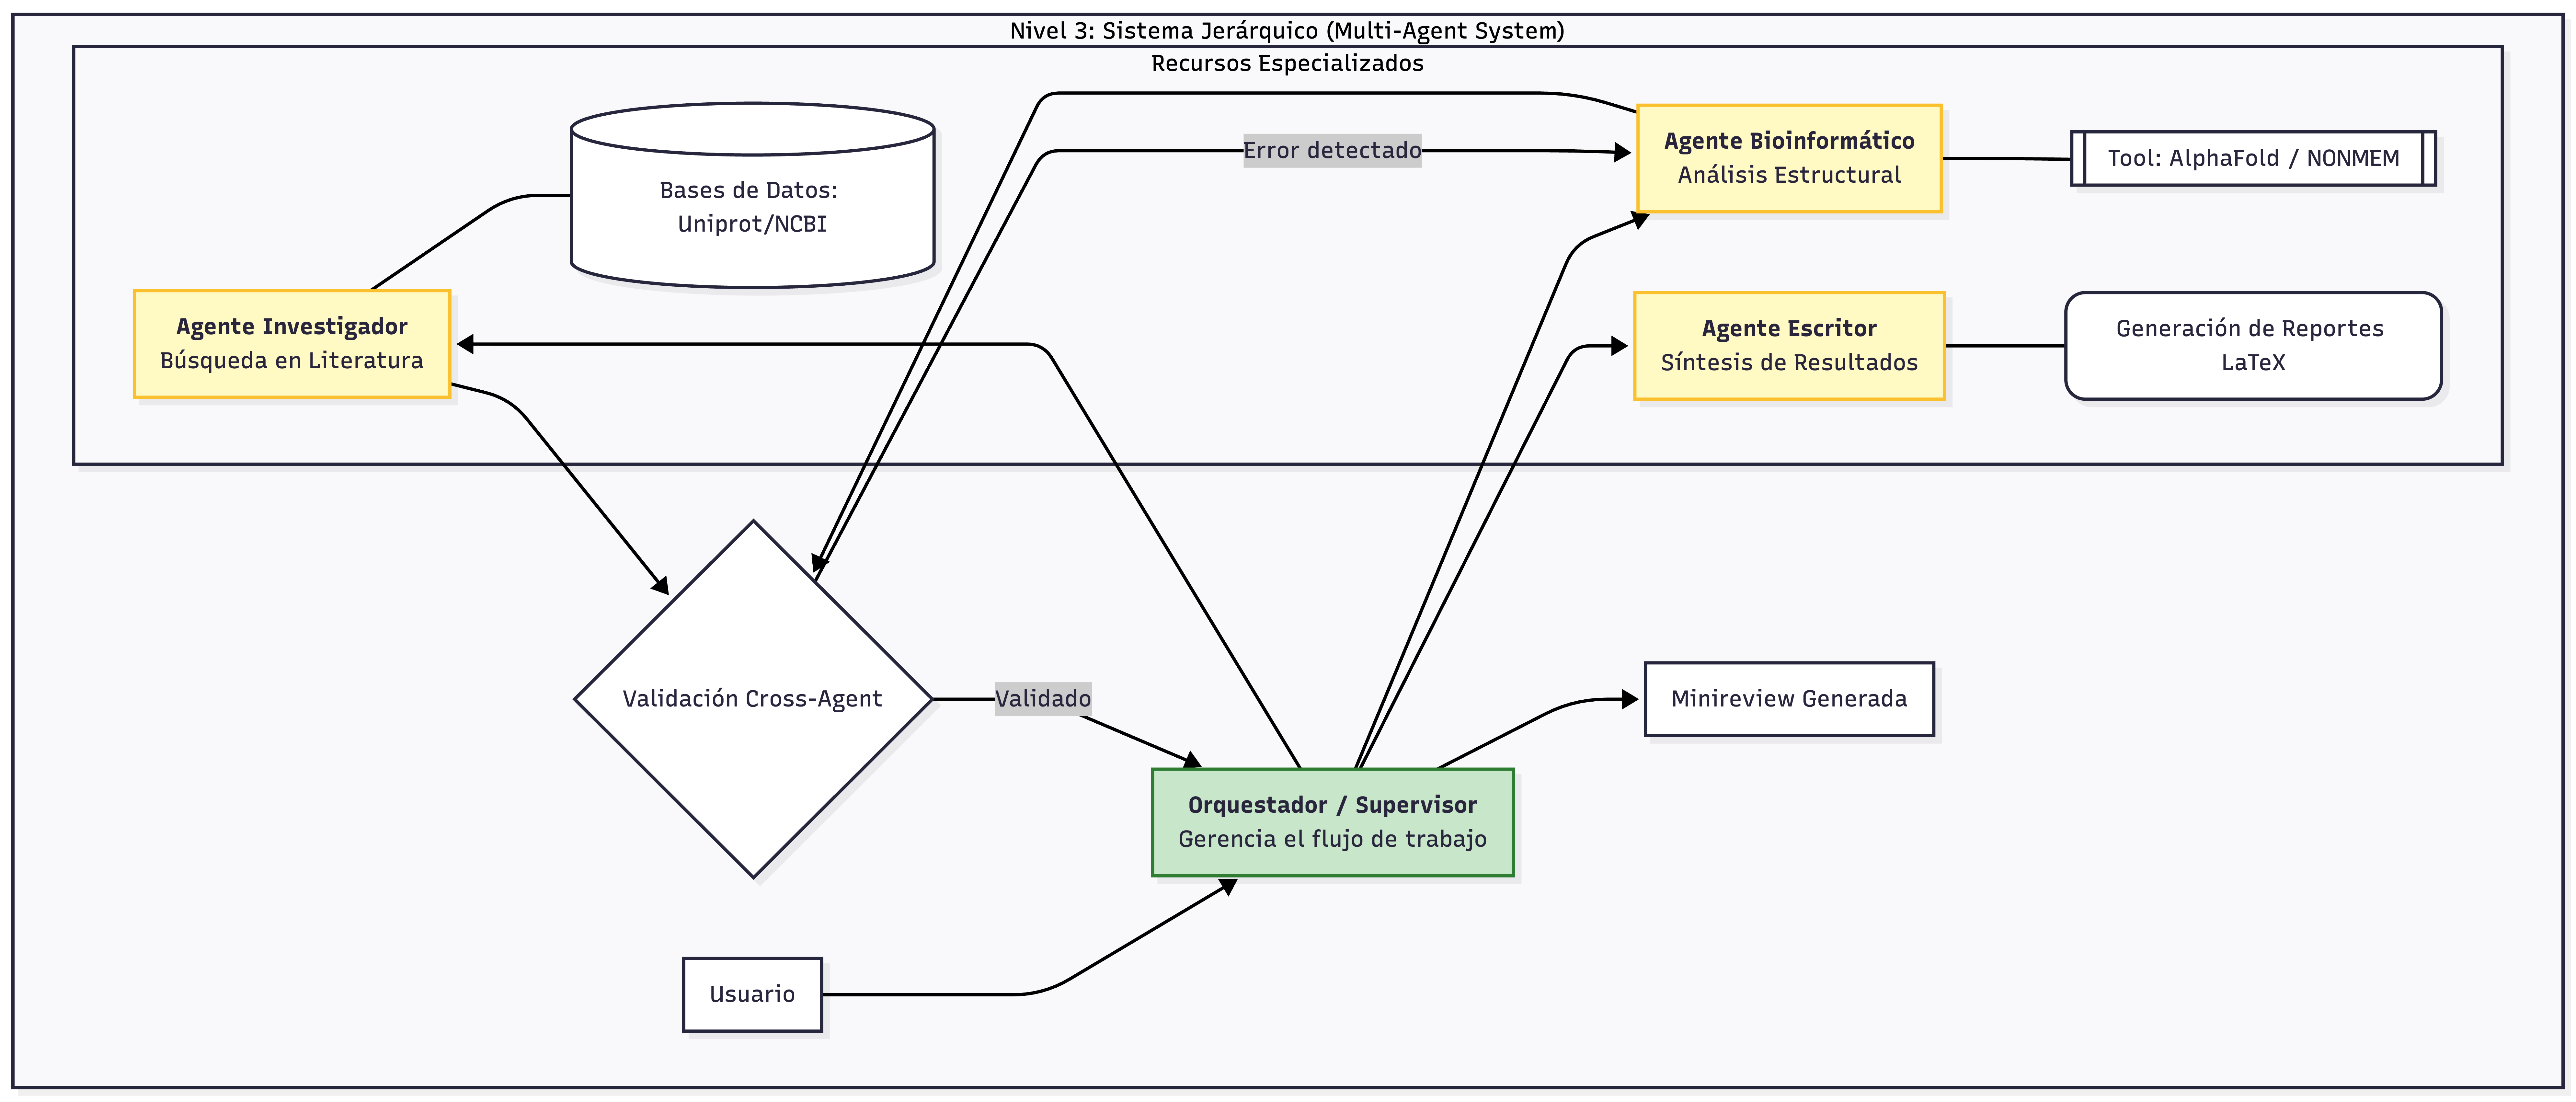
\includegraphics[width=\linewidth]{arquitectura_agentica.png}
    \caption{Arquitectura agéntica}
    \label{fig:agentic-architecture}
  \end{subfigure}
  \caption{Evolución conceptual desde modelos LLM usados mediante
  \textit{prompting} directo hacia agentes con herramientas y arquitecturas
  agénticas capaces de planificar, ejecutar, validar y refinar workflows
  científicos.}
  \label{fig:agentic-levels}
\end{figure}

% --- CAJA DE INFORMACIÓN (INFOBOX) ---
\begin{infobox}[Recuadro 1 \textbar{} Concepto clave]
  Un sistema agéntico combina razonamiento, planificación, memoria operativa,
  uso de herramientas externas y ciclos de retroalimentación. Esta arquitectura
  permite que el LLM deje de funcionar como un generador aislado de texto y pase
  a actuar como coordinador de un workflow computacional verificable.
  
  En bioinformática, esta separación entre razonamiento y ejecución es crítica
  porque permite delegar tareas técnicas a software especializado mientras se
  mantiene una capa de supervisión y validación.
\end{infobox}


Ejemplo de workflow en Python:

\begin{lstlisting}[style=python, caption={Workflow en Python con una libreria
  de LLMs, como LangChain u OpenAI API.}, label=lst:python_example]
from langchain.llms import OpenAI
from langchain.agents import initialize_agent, Tool

# Inicializar LLM
llm = OpenAI(temperature=0.0, model="gpt-4")

# Definir herramientas bioinformaticas
tools = [
    Tool(
        name="PubMedSearch",
        func=search_pubmed,
        description="Buscar articulos relevantes en PubMed"
    ),
    Tool(
        name="ParseSequence",
        func=parse_fasta,
        description="Procesar archivos de secuencias FASTA"
    ),
]

# Crear agente
agent = initialize_agent(tools, llm, agent="zero-shot-react-description")
result = agent.run("Buscar articulos sobre aplicaciones de CRISPR")
\end{lstlisting}

% --- CAJA DE PUNTO CLAVE (KEYPOINT) ---
\begin{keypoint}[Hallazgo clave del eje 1]
  La transición desde prompting directo hacia arquitecturas agénticas permite
  que los LLMs coordinen herramientas externas, ejecuten procesos iterativos y
  estructuren mejor el workflow científico, aunque la validación humana sigue
  siendo necesaria en tareas de alta sensibilidad biológica o clínica.
\end{keypoint}


% --- SUBSECCIÓN 2 ---
\subsection{Automatización de pipelines bioinformáticos específicos}\label{subsec:pipeline-automation}

Una parte significativa de los estudios seleccionados se enfocó en la
automatización de workflows computacionales en áreas como transcriptómica,
\textit{single-cell omics}, modelado farmacocinético y generación automatizada
de protocolos experimentales.

Sistemas como \textit{CellVoyager}~\citep{41845065} demostraron la capacidad de
los agentes para proponer análisis, ejecutarlos y producir resultados de forma
autónoma dentro de notebooks computacionales, especialmente en escenarios de
\textit{single-cell omics}. Otros trabajos mostraron la generación automática
de pipelines multi-step para virología y workflows de análisis ómicos,
reduciendo la intervención manual en tareas repetitivas y de ensamblaje
técnico~\citep{41523654}.

Además, algunos estudios extendieron estas capacidades hacia entornos wet-lab,
traduciendo información contenida en artículos científicos en protocolos
experimentales ejecutables.

\begin{figure}[htbp]
  \centering
  
\includegraphics[width=0.88\textwidth]{workflow.png}
  \caption{Representación conceptual de un workflow bioinformático automatizado
  mediante sistemas agénticos.}
  \label{fig:automated-workflow}
\end{figure}

Un aspecto crítico en esta automatización es la transición hacia workflows de
ciclo cerrado (\textit{closed-loop}). A diferencia de los scripts estáticos,
agentes como \textit{CellVoyager}~\citep{41845065} operan en entornos de ejecución dinámica,
como Jupyter Notebooks, donde el éxito de una tarea depende de la
retroalimentación inmediata del intérprete de código. Esta capacidad de
autocorrección amplía el alcance de procesos complejos, como el análisis de
\textit{single-cell omics}, y desplaza parte de la carga técnica desde el
investigador hacia el sistema, aunque no elimina por completo la necesidad de
revisión experta sobre la interpretación final.

% --- TABLA COMPARATIVA (TABULARX) ---
\begin{table}[H]
  \centering
  \small
  \caption{Comparación de sistemas, herramientas o enfoques evaluados en los estudios.}
  \label{tab:comparison}
  \begin{tabularx}{\textwidth}{@{} l l Y Y @{}}
    \toprule
    \textbf{Sistema} & \textbf{Enfoque} & \textbf{Dominio} &
    \textbf{Contribución principal} \\
    \midrule
    CellVoyager & Agente autónomo & \textit{Single-cell omics} &
    Ejecución autónoma de análisis y generación de hallazgos en notebooks. \\
    PKGPT & Agente recursivo & Farmacometría &
    Refinamiento iterativo de modelos NONMEM mediante ejecución externa y evaluación repetida. \\
    ChatSpatial & Orquestación por esquemas & Transcriptómica espacial &
    Reproducibilidad de workflows entre entornos R y Python mediante esquemas validados. \\
    Alvessa & Asistente con \textit{grounding} & Genómica funcional &
    Verificación a nivel de sentencia y trazabilidad de evidencia. \\
    \bottomrule
  \end{tabularx}
\end{table}

% --- SUBSECCIÓN 3 ---
\subsection{Reproducibilidad, benchmarking y evaluación comparativa}\label{subsec:reproducibility}

La reproducibilidad fue identificada como uno de los principales desafíos
asociados al uso de sistemas basados en agentes dentro de bioinformática.
Diversos estudios propusieron mecanismos para mejorar la trazabilidad,
consistencia y verificabilidad de los workflows automatizados.

\textit{ChatSpatial}~\citep{41890081} introdujo estrategias de orquestación basadas en esquemas
estructurados para mejorar la consistencia entre entornos R y Python, mientras
que otros trabajos propusieron asistentes basados en evidencia y mecanismos de
\textit{grounding} para reducir alucinaciones y mejorar la procedencia de la
información~\citep{41502944}.

De igual manera, algunos estudios desarrollaron frameworks de benchmarking
orientados a evaluar la calidad de generación de código, la ejecución de tareas
analíticas y la robustez de distintas capacidades agénticas en workflows
bioinformáticos complejos.

\begin{figure}[!t]
  \centering
  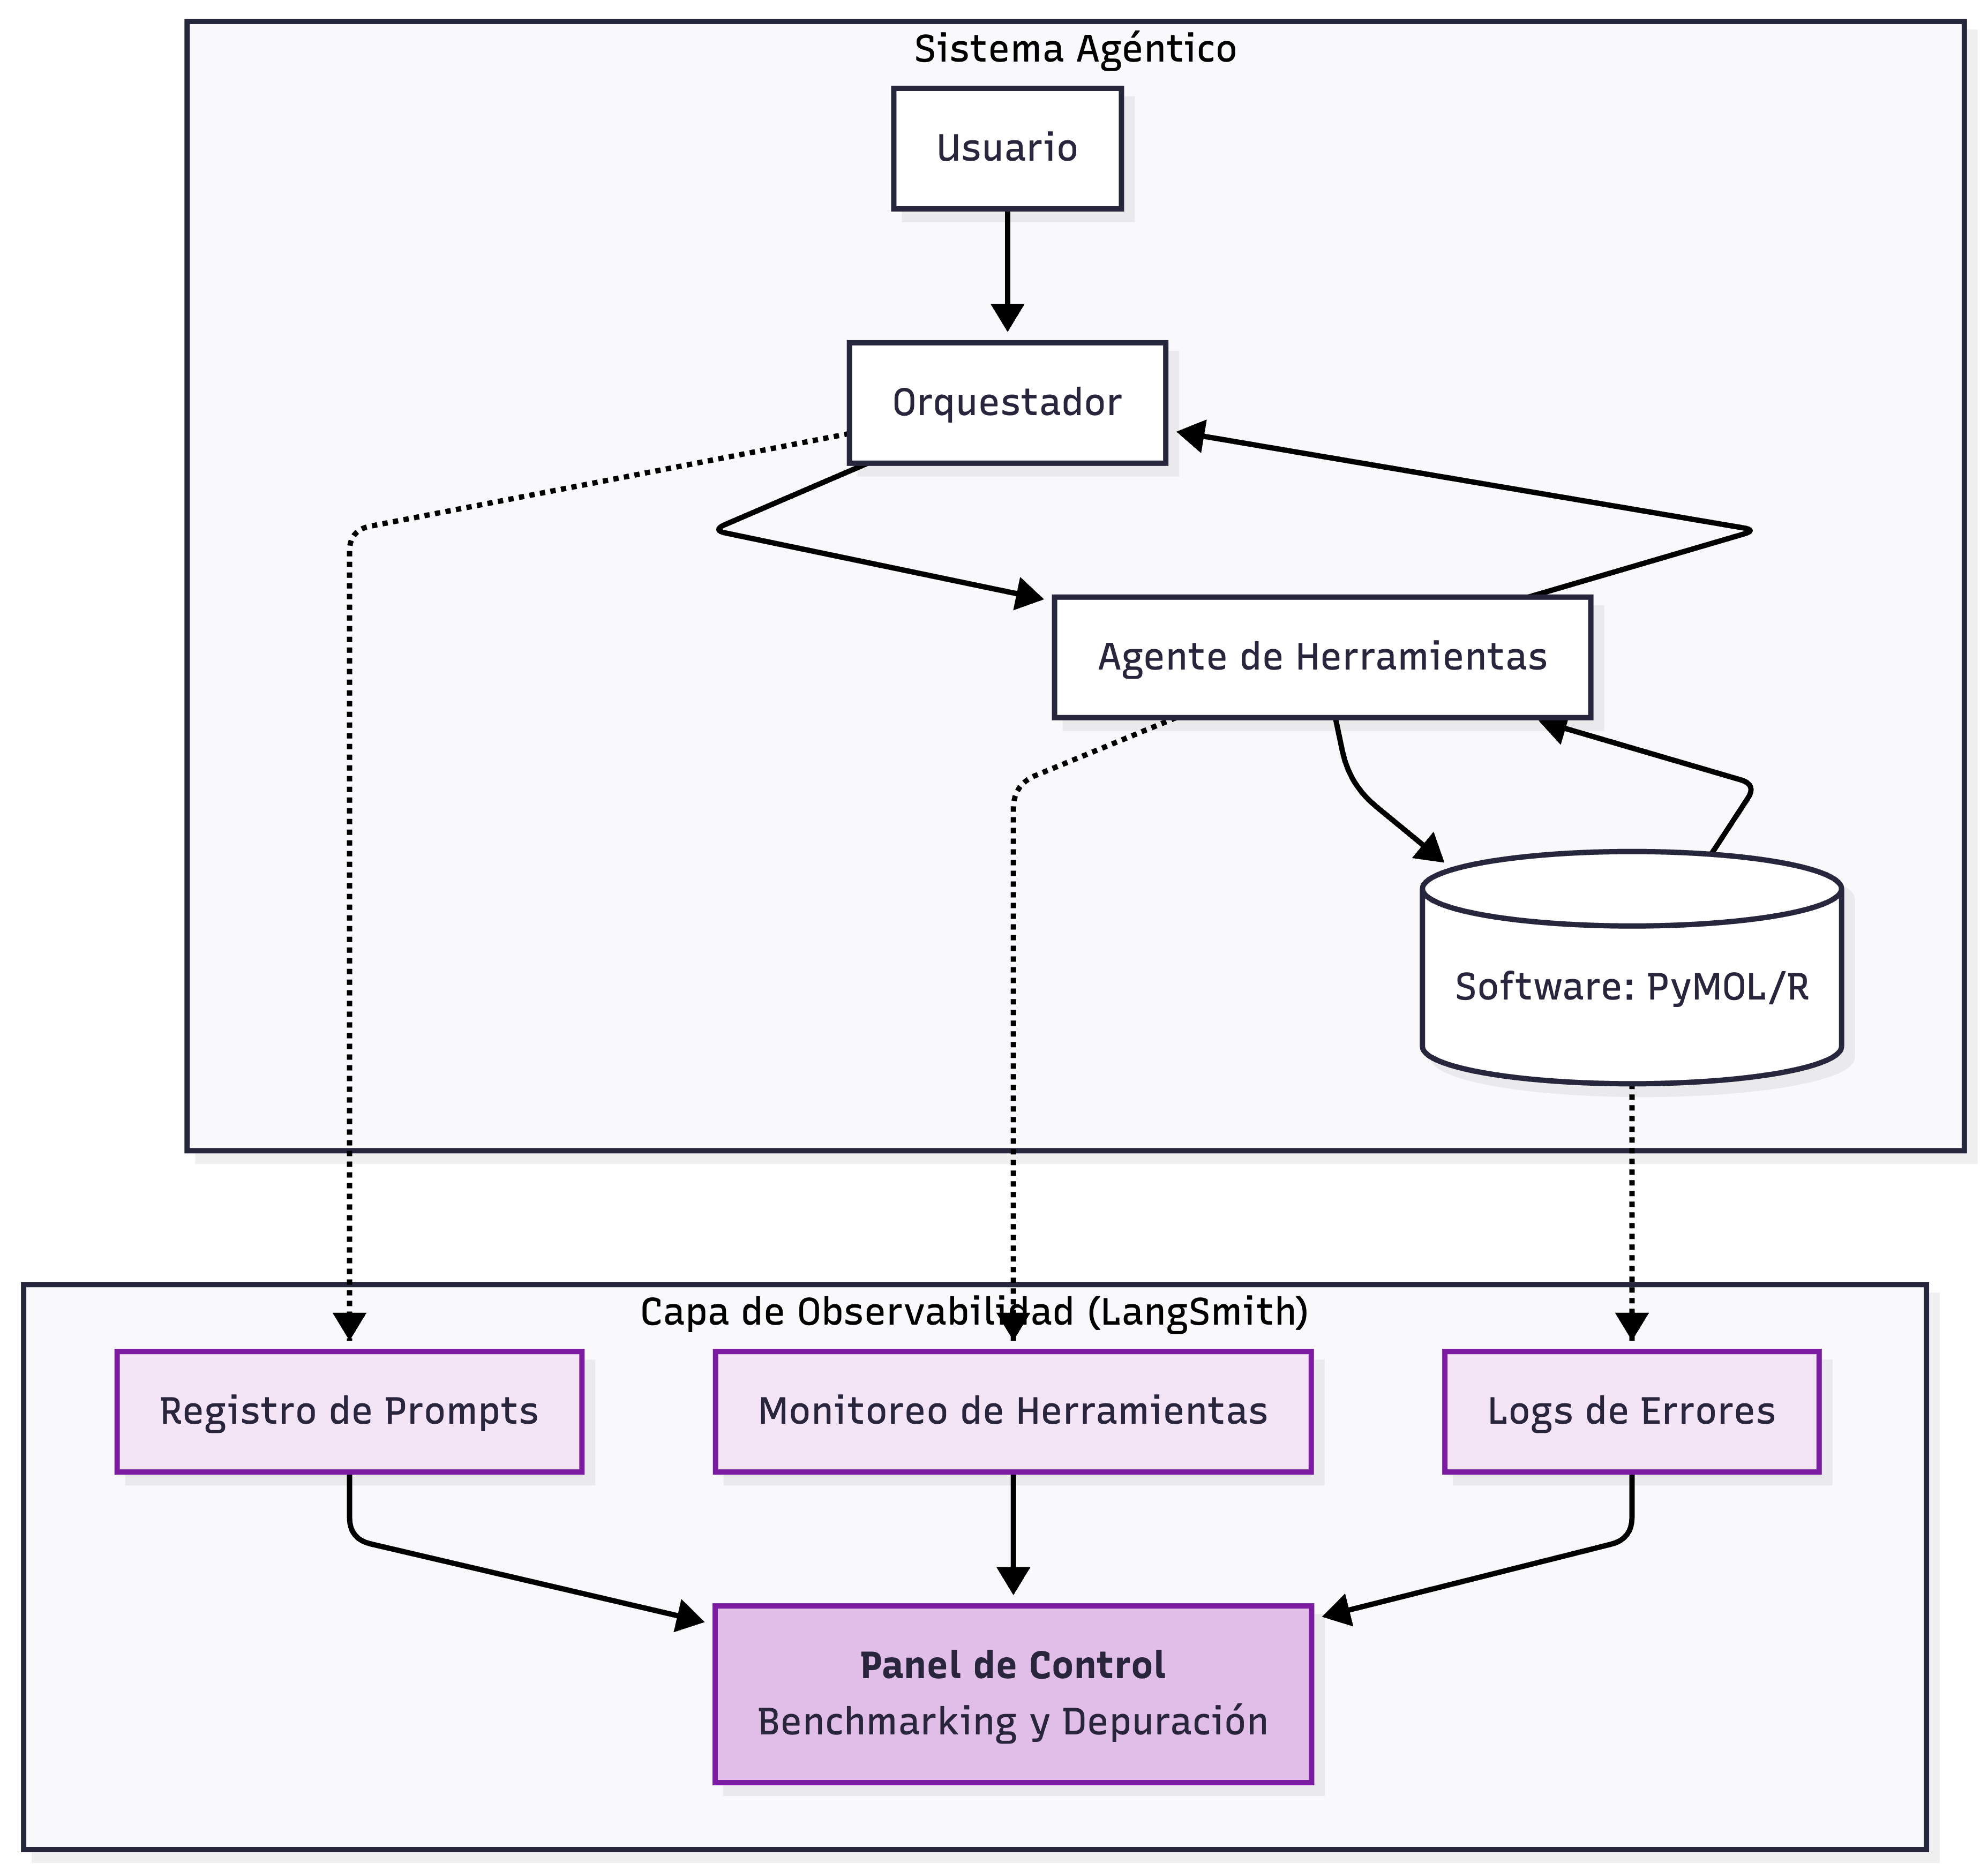
\includegraphics[width=0.80\textwidth]{observabilidad.png}
  \caption{Observabilidad de sistemas agénticos para auditoría de trazas,
  grafos de ejecución y consumo de recursos en workflows automatizados.}
  \label{fig:observability}
\end{figure}

Finalmente, la adopción de herramientas de observabilidad como
LangSmith~\citep{LangSmithObservability2026,LangSmithConcepts2026} puede ser
especialmente útil para fortalecer la robustez de estos sistemas. Estas
plataformas permiten una auditoría granular de los grafos de ejecución,
facilitando la identificación de cuellos de botella y errores de razonamiento
en flujos multi-agente, lo que eleva el estándar de reproducibilidad al permitir
que investigadores externos inspeccionen cada paso lógico y el consumo de
recursos de los experimentos automatizados.


% --- SUBSECCIÓN 4 ---
\subsection{Limitaciones técnicas y consideraciones de gobernanza}\label{subsec:governance}

A pesar del potencial observado en los sistemas basados en LLMs y agentes, la
literatura revisada reportó múltiples limitaciones relacionadas con
alucinaciones, coste computacional, dependencia de herramientas externas y
problemas de reproducibilidad.

Varios estudios señalaron que los LLMs presentan tasas de error significativas
durante ejecuciones iniciales, haciendo necesaria la incorporación de mecanismos
de validación iterativa, autocorrección y supervisión humana. Asimismo, el
elevado consumo de recursos computacionales y coste asociado al uso continuo de
modelos avanzados representa una barrera importante para su adopción
generalizada.

Finalmente, diferentes autores enfatizaron la ausencia de estándares claros para
la gobernanza y evaluación de sistemas agénticos en entornos científicos,
destacando la necesidad de desarrollar marcos normativos, estrategias de
supervisión humana y protocolos de validación reproducibles para futuras
implementaciones en bioinformática.

\begin{figure}[htbp]
  \centering
  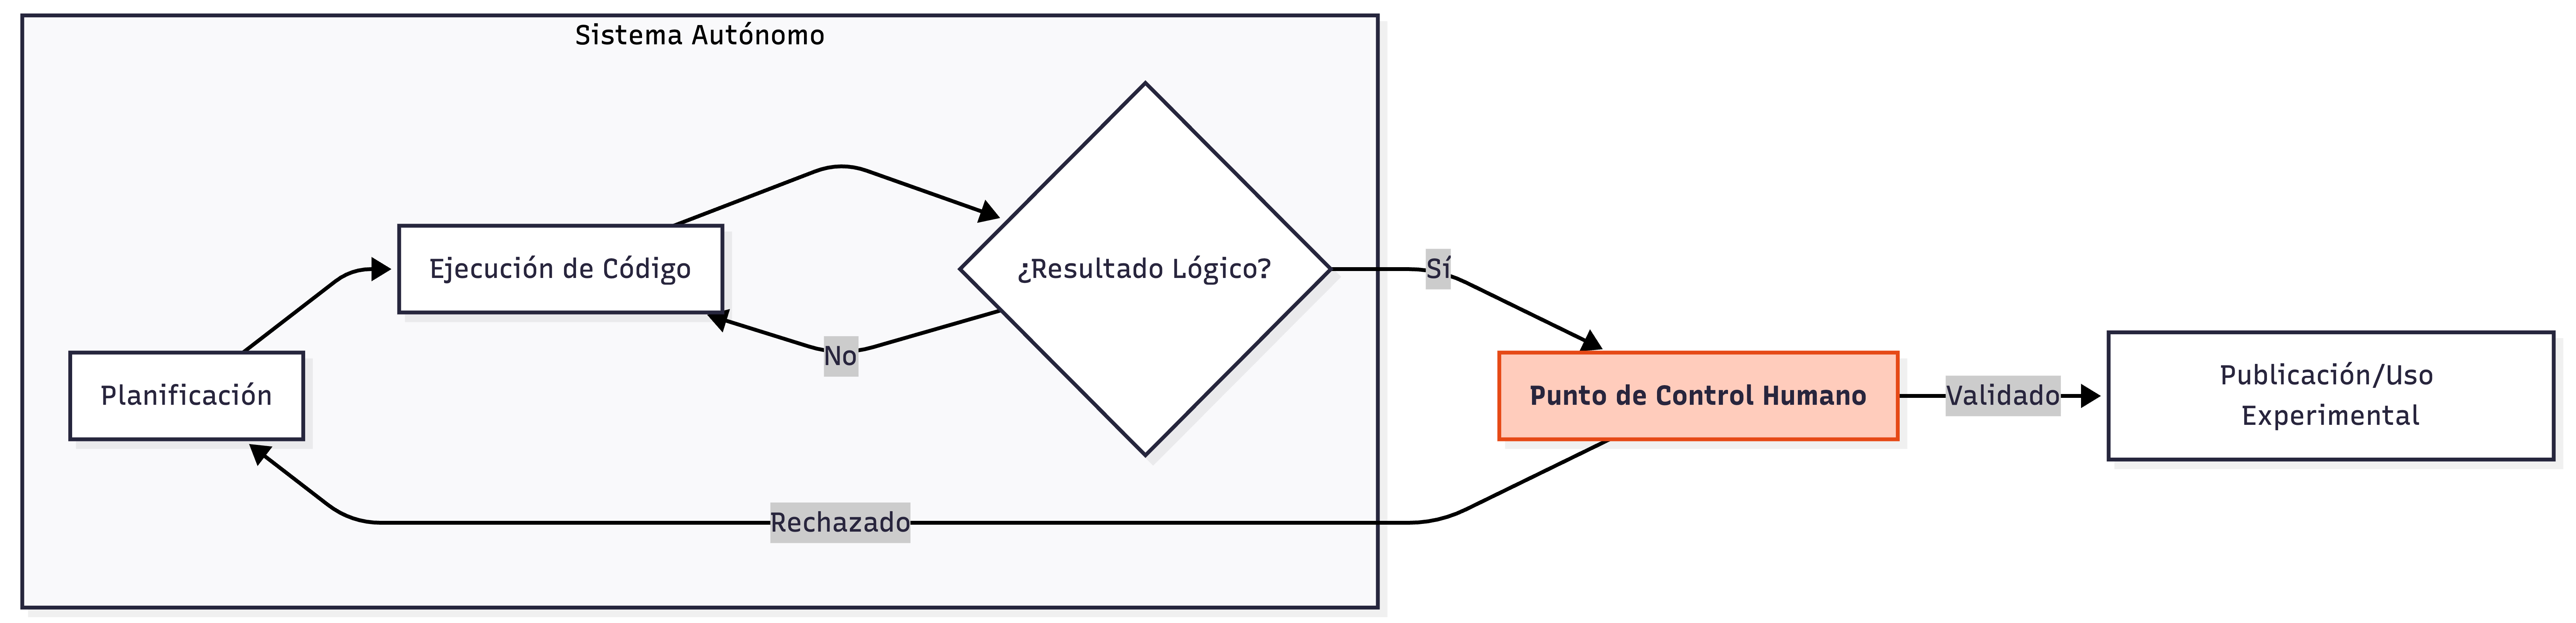
\includegraphics[width=0.88\textwidth]{riesgos.png}
  \caption{La supervisión humana y la observabilidad son componentes críticos
  del workflow agéntico: permiten intervenir en puntos de validación, auditar
  decisiones intermedias y mantener el control experimental durante la
  ejecución de pipelines bioinformáticos automatizados.}
  \label{fig:risks-governance}
\end{figure}

\begin{table}[htbp]
  \centering
  \caption{Limitaciones técnicas y estrategias de mitigación para sistemas
  agénticos en bioinformática.}
  \label{tab:limitations-governance}
  \begin{tabularx}{\textwidth}{@{} l X X @{}}
    \toprule
    \textbf{Categoría} & \textbf{Limitación técnica} &
    \textbf{Estrategia de mitigación} \\
    \midrule
    Fiabilidad &
    Alucinaciones en rutas metabólicas o secuencias. &
    \textit{Grounding} y verificación a nivel de sentencia
    (\textit{Alvessa}~\citealp{41502944}). \\
    Arquitectura &
    Errores en cascada en flujos multi-agente. &
    Implementación de \textit{unit testing} y observabilidad
    (LangSmith~\citealp{LangSmithObservability2026}). \\
    Coste &
    Elevado consumo de tokens en ciclos recursivos. &
    Uso de modelos \textit{small-language} (SLMs) para tareas de soporte. \\
    Gobernanza &
    Falta de trazabilidad en decisiones autónomas. &
    Protocolos de \textit{human-in-the-loop} en puntos críticos de validación. \\
    Interoperabilidad &
    Incompatibilidad entre herramientas biológicas. &
    Estandarización mediante el \textit{Model Context Protocol}
    (MCP~\citealp{41729821}). \\
    \bottomrule
  \end{tabularx}
\end{table}

La literatura sugiere que el despliegue de estos sistemas debe estar regido por
un marco de gobernanza clínica y técnica. Un desafío crítico es el ``coste de la
autonomía''; por ejemplo, sistemas que utilizan razonamiento recursivo pueden
consumir entre 15 y 50 veces más tokens que un enfoque \textit{zero-shot}. Para
mitigar esto, se propone la integración de capas de observabilidad que permitan
monitorizar el presupuesto de tokens en tiempo real. Además, la gobernanza debe
incluir protocolos de validación humana obligatoria antes de la transición de un
flujo computacional (\textit{in silico}) a uno experimental (\textit{in vitro}),
asegurando que la IA actúe como un copiloto de alta velocidad y no como un
tomador de decisiones final sin supervisión.

% ==============================================================================
% SECTION 4: DISCUSSION
% ==============================================================================

\section{Discusión}\label{sec:discussion}

\subsection{Hallazgos principales}\label{subsec:main-findings}

Los hallazgos de esta revisión subrayan que los sistemas agénticos no son solo
una mejora incremental, sino un cambio de paradigma en la bioinformática
computacional. Se identificó que la autocorrección iterativa es el componente
vital que permite la automatización de tareas que anteriormente requerían
supervisión humana constante, como el modelado PopPK o ciertos análisis de
\textit{single-cell omics}, aunque la validación experta continúa siendo
necesaria en etapas críticas.

Un hallazgo fundamental es el valor de la orquestación jerárquica, donde un
agente supervisor coordina a especialistas en herramientas y distribuye tareas
analíticas de forma más estructurada. No obstante, los resultados también
revelan que la calidad de los prompts de sistema y la estructura de las
herramientas disponibles, es decir, herramientas agénticas o legibles por
máquina, son determinantes centrales del éxito del workflow.

Este patrón valida la necesidad de protocolos como el \textit{Model Context
Protocol} (MCP) para el futuro del área, ya que la interoperabilidad entre
agentes, herramientas bioinformáticas y entornos de ejecución científica emerge
como una condición central para escalar estos sistemas de forma reproducible.

\subsection{Limitaciones}\label{subsec:discussion-limitations}

A pesar del potencial disruptivo, la implementación de agentes en
bioinformática enfrenta barreras técnicas críticas. El comportamiento no
determinista de los modelos subyacentes introduce una variabilidad inaceptable
en flujos de trabajo que requieren precisión absoluta, como el modelado PopPK.
Asimismo, la propagación de errores en arquitecturas jerárquicas, donde una
alucinación inicial contamina las etapas subsiguientes, subraya la inmadurez de
los mecanismos de autocorrección actuales.

La literatura también destaca la ausencia de estándares de diseño, lo que genera
una fragmentación de herramientas que dificulta la interoperabilidad. Finalmente,
la reproducibilidad sigue siendo un desafío abierto; la naturaleza de ``caja
negra'' de los LLMs comerciales impide asegurar que un experimento automatizado
produzca resultados idénticos en el tiempo, lo que requiere una transición hacia
modelos locales y registros de observabilidad más estrictos.

\begin{itemize}
  \item \textbf{Comportamiento no determinista:} Los LLMs pueden generar
  respuestas distintas ante el mismo prompt, lo que en bioinformática es
  crítico. Un agente puede proponer un script de PyMOL funcional hoy y uno con
  errores de sintaxis mañana. Esto obliga a implementar capas de validación de
  esquemas, como propone \textit{ChatSpatial}, para forzar una estructura en la
  salida.

  \item \textbf{Propagación de errores:} En sistemas multi-agente, si el agente
  investigador extrae un dato erróneo de PubMed, el agente programador escribirá
  código basado en ese error y el agente analista generará conclusiones falsas.
  Sin un monitor de errores, como
  LangSmith~\citep{LangSmithObservability2026,LangSmithConcepts2026}, este
  error puede permanecer invisible hasta el final del flujo.

  \item \textbf{Falta de estándares de diseño:} Actualmente no existe un
  lenguaje universal para que los agentes interactúen con herramientas
  bioinformáticas. Cada desarrollador crea sus propias funciones de Python. Aquí
  surge la necesidad del \textit{Model Context Protocol}
  (MCP)~\citep{41729821} para estandarizar la invocación de herramientas
  bioinformáticas externas por parte de agentes.

  \item \textbf{Dificultad en la reproducibilidad:} Debido a la actualización
  constante de modelos comerciales, un workflow agéntico documentado en 2025
  podría no funcionar igual en 2026, lo que desafía los principios de la ciencia
  abierta y dificulta la revisión por pares.
\end{itemize}

\begin{table}[htbp]
  \centering
  \caption{Impacto de las principales limitaciones de los sistemas agénticos en
  bioinformática y estrategias de mitigación sugeridas.}
  \label{tab:discussion-limitations}
  \begin{tabularx}{\textwidth}{@{} l X X @{}}
    \toprule
    \textbf{Limitación} & \textbf{Impacto en bioinformática} &
    \textbf{Mitigación sugerida} \\
    \midrule
    No determinismo &
    Variabilidad en resultados de simulaciones. &
    Fijación de temperatura ($T=0$) y \textit{prompt engineering} robusto. \\
    Propagación &
    Alucinaciones científicas verosímiles. &
    Mecanismos de \textit{grounding} y validación cruzada entre agentes. \\
    Falta de estándares &
    Fragmentación de herramientas y silos. &
    Adopción de protocolos de interoperabilidad, como
    MCPmed~\citealp{41729821}. \\
    Reproducibilidad &
    Imposibilidad de replicar pipelines exactos. &
    Registro exhaustivo de versiones y trazas de ejecución, como
    LangSmith~\citealp{LangSmithObservability2026}. \\
    \bottomrule
  \end{tabularx}
\end{table}

\subsection{Vacíos en la literatura}\label{subsec:literature-gaps}

La revisión identifica vacíos críticos que limitan la adopción masiva de estas
tecnologías. En primer lugar, la falta de benchmarks estandarizados impide una
comparación justa entre las crecientes arquitecturas agénticas, relegando la
evaluación a éxitos anecdóticos en lugar de métricas universales.

En segundo lugar, existe una carencia de evaluaciones comparativas rigurosas que
analicen la relación entre el costo computacional y la ganancia en precisión
científica, un factor determinante para la sostenibilidad en el entorno
académico. Finalmente, la ausencia de estudios en entornos reales deja abierta
la capacidad de estos sistemas para manejar ambigüedad y requisitos de
seguridad sobre datos genómicos sensibles.

Cerrar estos vacíos será clave para pasar de prototipos experimentales a
sistemas de producción científica confiables.

% ==============================================================================
% SECTION 5: CONCLUSIONS
% ==============================================================================

\section{Conclusiones}\label{sec:conclusions}

\subsection{El cambio de paradigma: de LLMs a sistemas agénticos}
\label{subsec:paradigm-shift}

La revisión de la literatura permite concluir que los modelos de lenguaje por sí
solos son insuficientes para las demandas de la bioinformática debido a su
naturaleza probabilística. Sin embargo, la transición hacia sistemas agénticos,
que integran razonamiento, uso de herramientas externas y ciclos de
retroalimentación, ha demostrado ser un avance disruptivo.

Estos sistemas no solo ``escriben'' código, sino que actúan como agentes
ejecutores capaces de iterar hasta alcanzar soluciones técnicas válidas, como se
observó en la automatización del modelado farmacocinético y el análisis de
\textit{single-cell omics}.

\subsection{La verificabilidad como requisito científico}
\label{subsec:verifiability}

Un hallazgo crítico es que la autonomía no debe comprometer la integridad
científica. La implementación de estrategias de \textit{grounding} y
verificación a nivel de sentencia, como en el caso de Alvessa, es esencial para
transformar las alucinaciones de los modelos en resultados trazables.

La integración de herramientas de observabilidad como LangSmith se perfila no
como un lujo técnico, sino como una necesidad metodológica para garantizar la
auditoría y la reproducibilidad de los descubrimientos científicos generados por
IA.

\subsection{Perspectivas futuras y estandarización}
\label{subsec:future-standardization}

El futuro de la automatización en bioinformática depende de la creación de un
ecosistema interoperable. La adopción de protocolos como el \textit{Model
Context Protocol} (MCP) y el desarrollo de benchmarks especializados, por
ejemplo GenomeArena, serán los catalizadores que permitan pasar de prototipos
aislados a infraestructuras de investigación robustas.

A medida que se reduzcan los costes computacionales y mejore la precisión de los
agentes, estos sistemas se convertirán en colaboradores esenciales en el
laboratorio, permitiendo que el investigador humano se desplace de las tareas de
ejecución técnica hacia la formulación de hipótesis de alto nivel y la toma de
decisiones estratégicas.

En conclusión, los sistemas basados en agentes no solo automatizan tareas
repetitivas, sino que democratizan el acceso a flujos de trabajo bioinformáticos
complejos, siempre que su despliegue esté regido por marcos de gobernanza
transparentes, observabilidad estricta y una validación humana continua.


\newpage
\nocite{*}
\bibliography{references}

\end{document}
